\documentclass[10pt,a4paper]{article}
\usepackage[utf8]{inputenc}
\usepackage[english]{babel}
\usepackage[T1]{fontenc}
\usepackage{amsmath}
\usepackage{amsfonts}
\usepackage{amssymb}
\usepackage{subcaption}
\usepackage{makeidx}
\usepackage{graphicx}
\usepackage{fourier}
\usepackage{listings}
\usepackage{color}
\usepackage{hyperref}
\usepackage[left=2cm,right=2cm,top=2cm,bottom=2cm]{geometry}
\author{Tommy Müller, Marcus Dittrich, Vincent Noculak}
\title{Rastertunnelmikroskopie}

\lstset{language=C++,
	keywordstyle=\bfseries\color{blue},
	commentstyle=\itshape\color{red},
	stringstyle=\color{green},
	identifierstyle=\bfseries,
	frame=single}
\begin{document}

\maketitle
\newpage
\tableofcontents
\newpage

\section{Versuchsauswertung}

\subsection{Ebene Grafitoberfläche}

Zum Untersuchen der atomaren Struktur von Grafit, haben wir versucht eine ebene Fläche in unserer Probe zu finden und sie zu messen. Die Feinheit der zur Messung verwendeten Sensorspitze ist ausschlaggebend dafür, wie exakt Strukturen auf der Grafitoberfläche gemessen werden können. Weil wir die Spitze mit einer Zange, durch das abkneifen eines Drahtes, hergestellt haben, war die Wahrscheinlichkeit groß, dass der Sensor zum Messen der atomaren Struktur nicht fein genug ist. Obwohl wir ebene Flächen im Grafit fanden, war es nicht möglich atomare Strukturen zu erkennen.

 Deshalb haben wir zur Untersuchung der atomaren Struktur die Daten aus den Referenzmessungen verwendet. Die Messung aus den Referenzmaterialien kann in Abbildung \ref{Grafitoberflächenebene} gesehen werden. Hier ist \ref{grafob1} die rohe Messung an sich. Es ist die ebene Oberfläche des Grafits zu erkennen. In \ref{grafob2} haben wir mithilfe einer doppelten Fouriertransformation Störungen aus der Messung entfernt. Dadurch lässt sich die atomare Struktur genauer untersuchen.

\begin{figure}[h]
	\centering
	\begin{subfigure}{0.45\textwidth}
		\centering
		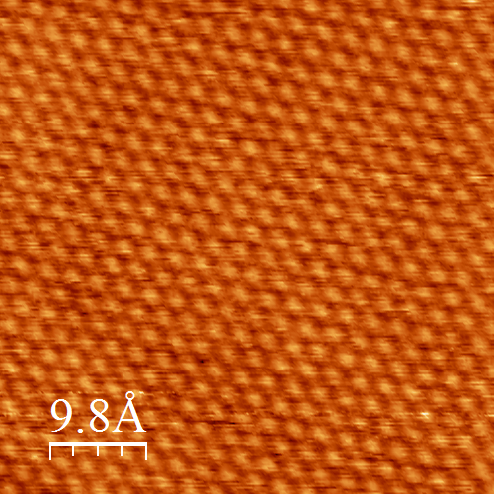
\includegraphics[width=\textwidth]{vor_doppelter_fourier.png}
		\caption{gemessene Grafitoberfläche}
		\label{grafob1}
	\end{subfigure}
	\begin{subfigure}{0.45\textwidth}
		\centering
		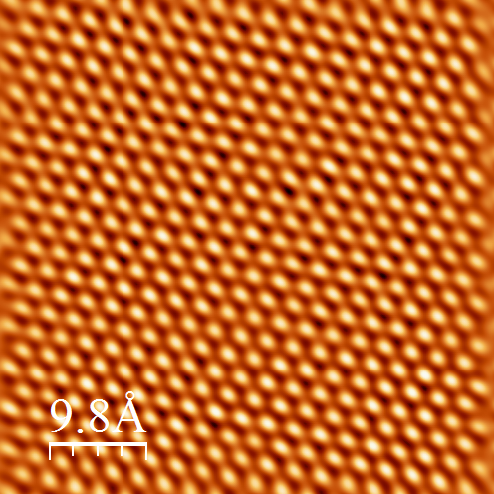
\includegraphics[width=\textwidth]{nach_doppelter_fourier.png}
		\caption{Gemessene Grafitoberfläche, nachdem Störungen durch eine doppelte Fouriertransformation beseitigt wurden}
		\label{grafob2}
	\end{subfigure}

	\caption{Messung des Tunnelstroms an einer ebenen Fläche Grafit}
	\label{Grafitoberflächenebene}
\end{figure}

Es kann klar erkannt werden, dass die Kohlenstoffatome regelmäßig in einer Kristallstruktur angeordnet sind. Man erkennt ein hexagonales Kristallsystem, wie es für Grafit zu erwarten war.

\begin{figure}[h]
	\centering

	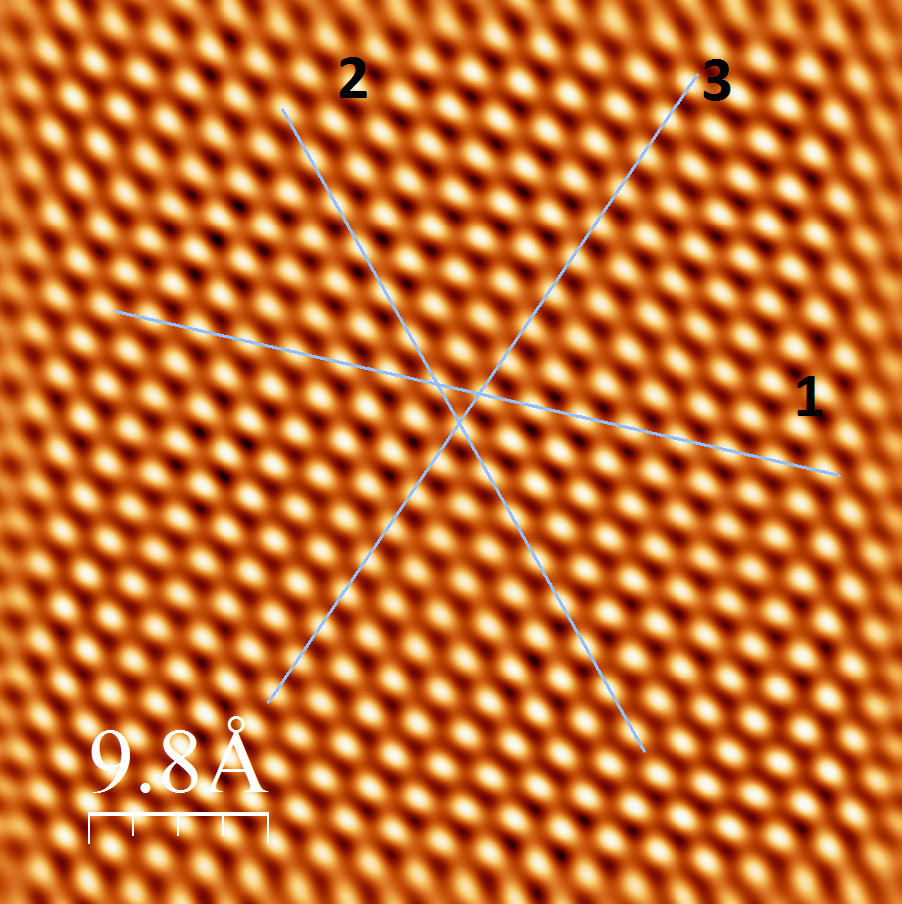
\includegraphics[scale = 0.4]{Aufnahme_Ebene_doppelte_fourier2.png}

	\caption{Messung der Abstände der atomaren Erhebungen}
	\label{Messungerh1}
\end{figure}

\subsubsection{Messungen an atomaren Erhebungen} \label{kapitolo}

Entlang der in \ref{Messungerh1} zu sehenden Geraden haben wir die Abstände der atomaren Erhebungen gemessen. Das dazugehörige Diagramm zu Gerade 1 kann in Abbildung \ref{Messungerh2} gesehen werden. Wir haben alle Abstände entlang der zu sehenden Geraden gemessen und anschließend einen Mittelwert mit Standardabweichung gebildet. Die gemessenen Abstände für alle atomaren Ausrichtungen sind in Tabelle \ref{Messungerh5} zu sehen. Unsere Werte für den Abstand der atomaren Erhebungen ist entlang Gerade 1 $(0,265 \pm 0,002) nm$, Gerade 2 $(0,273 \pm 0,002) nm$ und Gerade 3 $(0,222 \pm 0,003) nm$. Unsere durch die Standardabweichung erhaltenen Fehler von $0,002 nm$ beziehungsweise $0,003 nm$, sind kleiner, als es physikalisch sinnvoll wäre. Alleine der Fehler durch die Schwingung des Gitters, abhängig von der Temperatur sollte größer sein. Deshalb nehmen wir für unsere Fehler den Standardfehler der Messwerte. Damit sind unsere Werte für die Abstände der atomaren Erhebungen $(0,27 \pm 0,01) nm$, $(0,27 \pm 0,01) nm$ und $(0,22 \pm 0,01) nm$

Laut der Theorie sehen wir in dem mit dem Rastertunnelmikroskop aufgenommenen Bild nur jedes zweite Atom des Grafit-Kristalls. Der planare Abstand nächster Nachbarn im Kristall ist mit $b = 0,142 nm$ gegeben. Der von uns zu erwartende Abstand der atomaren Erhebungen lässt sich mithilfe des Kosinussatzes als 

\begin{equation}
	s = b \cdot \sqrt{2(1-cos(120^\circ))} = 0,246 nm
	\label{eq:aabstand}
\end{equation}

berechnen. Die Rechnung kann anhand von Abbildung \ref{rechnungatomabstand}, in der die hexagonale Struktur Grafits dargestellt ist, hergeleitet werden. Unsere Werte stimmen mit dem dritten Fehlerintervall mit dem theoretischen Wert überein. Hätten wir die Standardabweichung als Fehler genommen, würden unsere Werte über 10 Fehlerintervalle von dem theoretischen abweichen.

\begin{figure}[h]
	\centering
	
	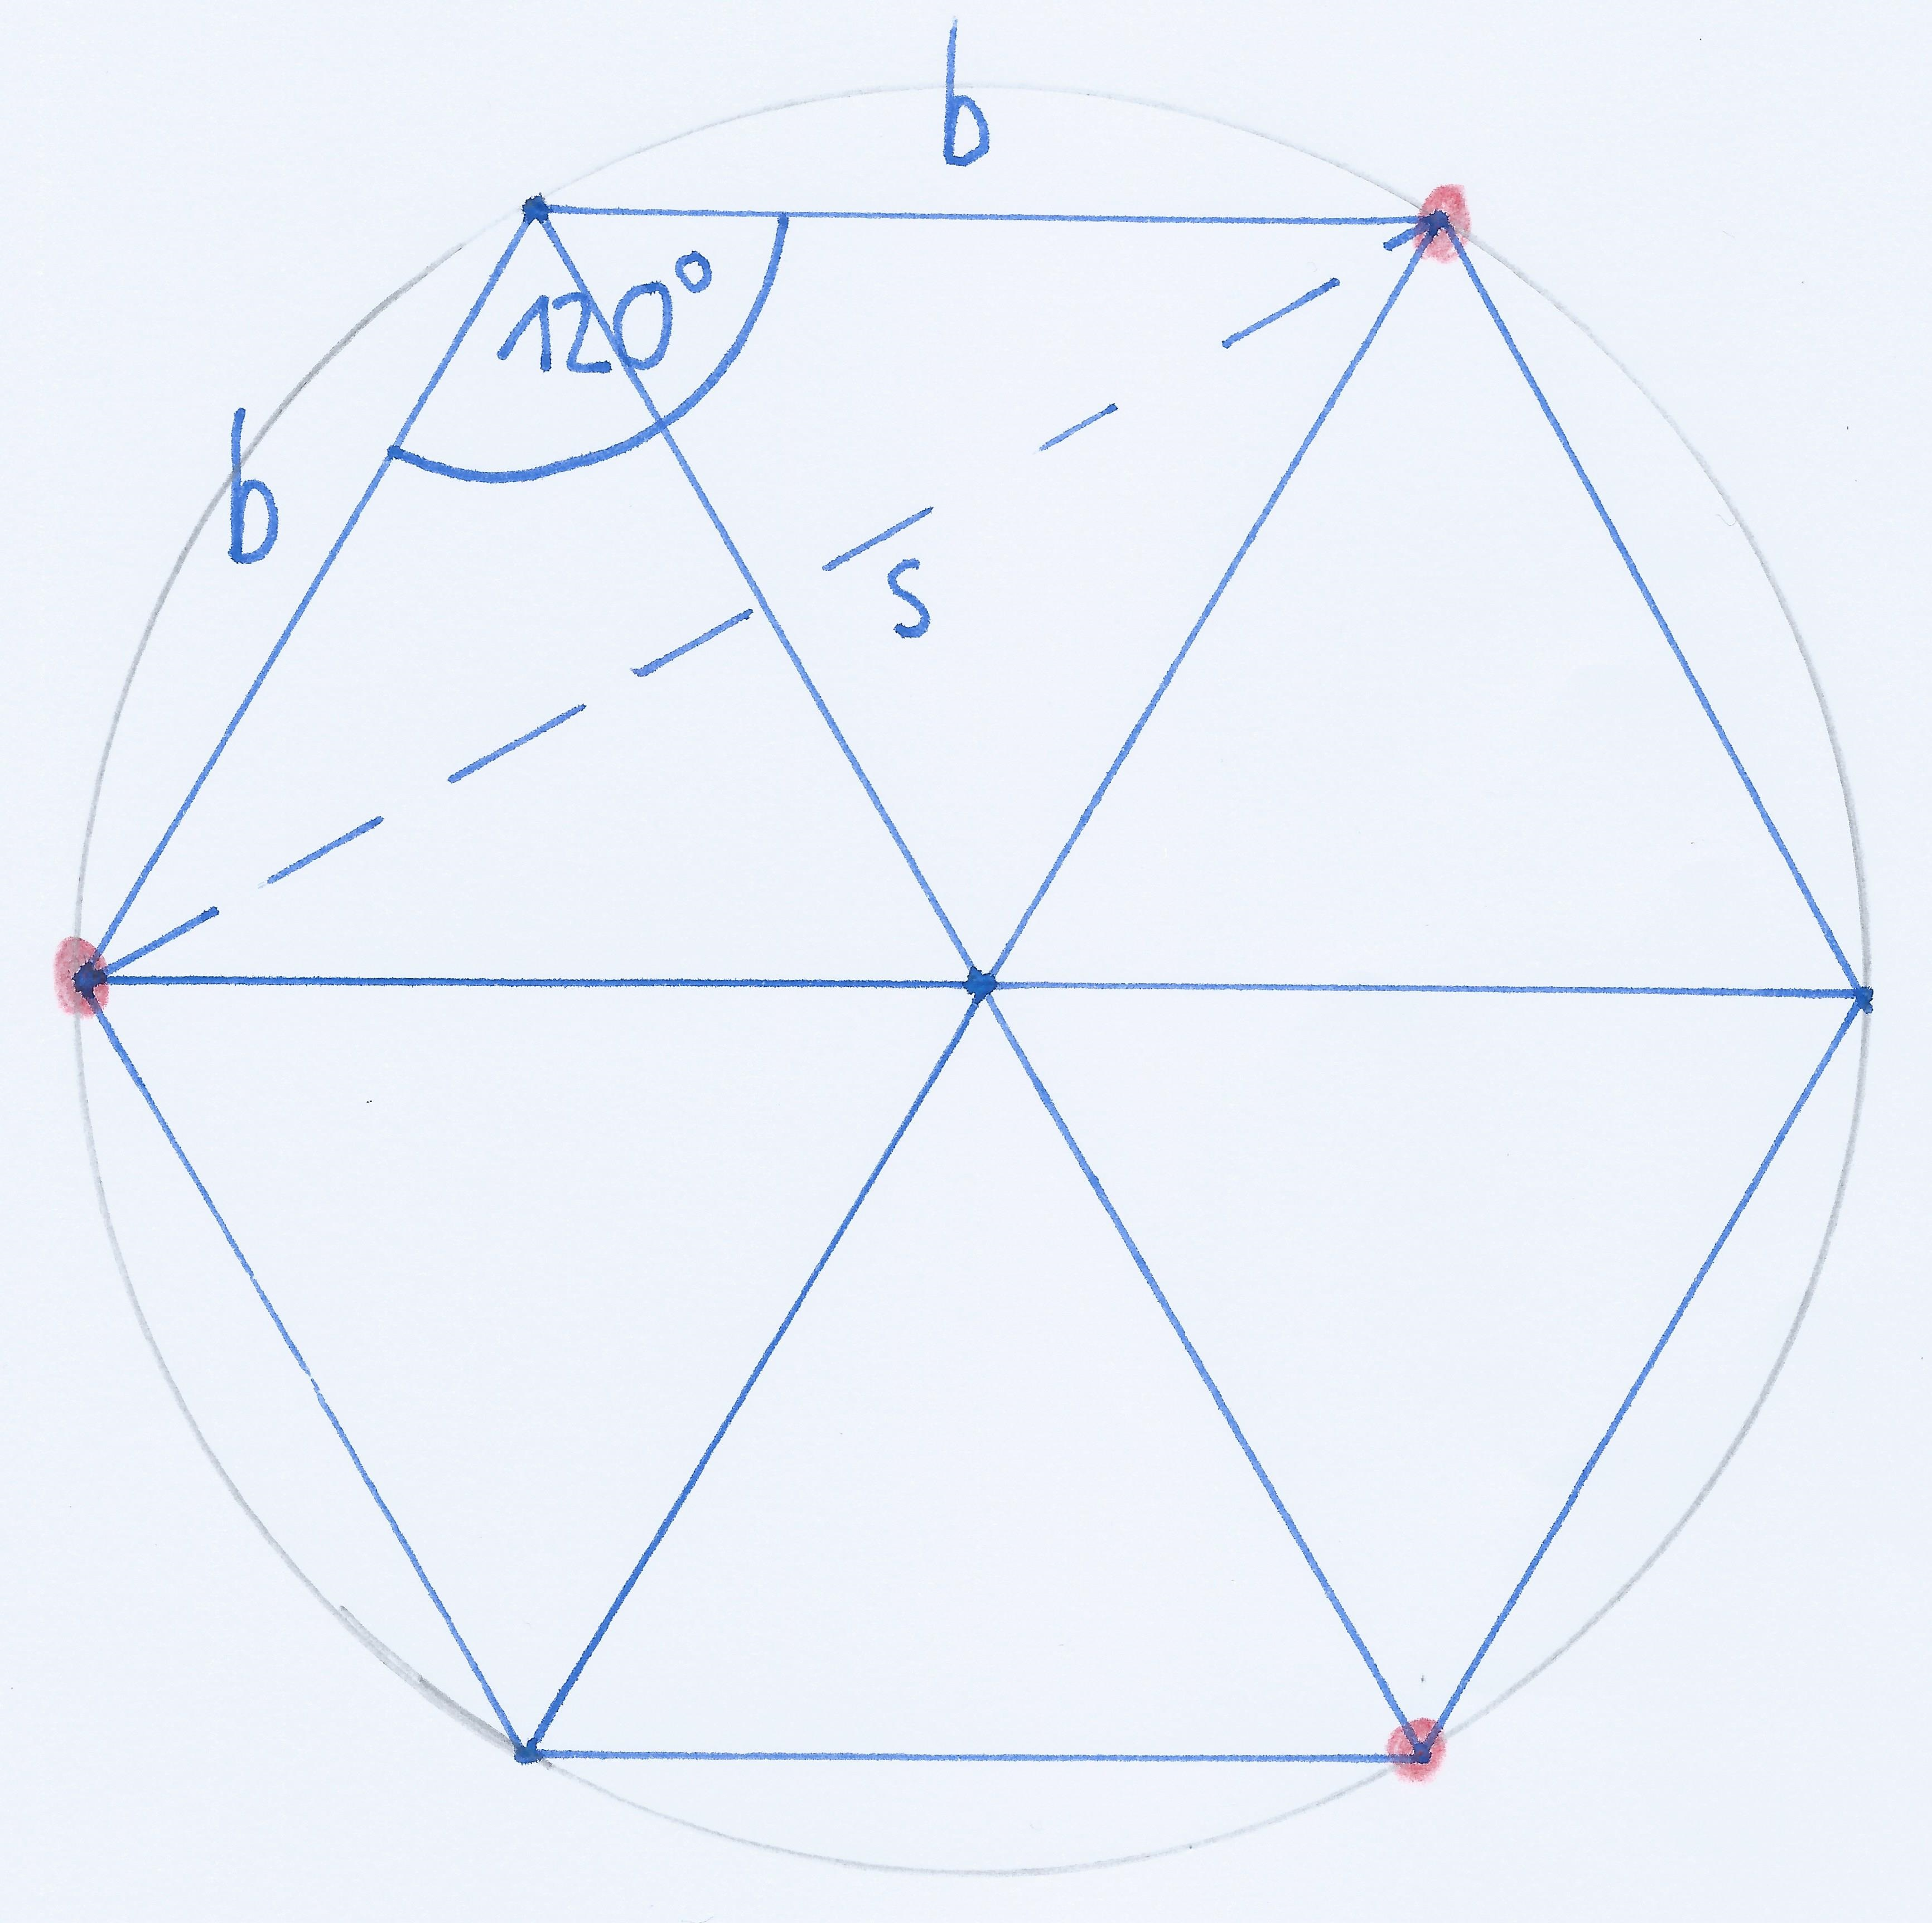
\includegraphics[scale = 0.4]{hexagon.jpg}
	
	\caption{Hexagonale Struktur des Grafits: Im Rastertunnelmikroskop sichtbare Atome sind rot gekennzeichnet}
	\label{rechnungatomabstand}
\end{figure}

Eine wichtige Größe, die großen Einfluss auf den Messfehler hat, ist die Temperatur während der Messung. Sie beeinflusst die Energie des Kristalls und somit auch seine Eigenbewegung. Eine weitere Fehlerquelle, dass unser Wert nicht mit dem theoretischen übereinstimmt wäre, dass wir mit dem Rastertunnelmikroskop nicht senkrecht zur Probe messen. Dieser Fehler ist jedoch so klein einzuschätzen, dass er nicht ausschlaggebend für die vom theoretischen Wert abweichenden Messwerte ist. Eine größere Fehlerquelle ist, dass der Sensor in einem Raster über die Ebene fährt. Dies tut er mit Hilfe von einem X- und Y-Piezoelement. Sind die Piezoelemente nicht richtig kalibriert, so kommt es in den Messbildern zu Verzerrungen. Diese Verzerrungen stellen einen systematischen Fehler dar, der erklären würde, weshalb alle von uns gemessenen Werte entlang einer atomaren Ausrichtung über beziehungsweise unter dem theoretischen Wert liegen (mehr zur Verzerrung durch die Piezoelemente in Kapitel \ref{winkelsec}). Daraus folgt, dass unser gemessener Wert möglicherweise mit dem theoretischen übereinstimmen könnte, wenn man den systematischen Fehler entfernen würde.  

Eine weitere Fehlerquelle, die eine Verzerrung des Messbildes verursachen könnte, ist eine Temperaturdifferenz zwischen Messspitze und Probe. Durch eine solche Temperaturdifferenz, würde die Messspitze mit der Probe durch Wärmetransport wechselwirken und somit das Messbild beeinflussen. Je länger der Sensor über einer Stelle der Probe sitzt, desto mehr Wärme wird zwischen Sensor und Probe ausgetauscht. Deshalb ist dieser Fehler besonders klein, wenn sich der Sensor schnell über die Probe bewegt. Zur Aufnahme unserer Messbilder bewegt sich der Sensor in einem Raster über die Probe. Weil er sich dabei die meiste Zeit in der horizontalen Achse der Messbilder bewegt, sollte die durch die Temperaturdifferenz auftretende Verzerrung in diese Richtung am geringsten sein. In unseren Messaufnahmen sollten deshalb, wenn der sogenannte thermische Drift der dominante Fehler ist, die atomaren Abstände entlang Gerade 1 am meisten den theoretischen entsprechen. Dies ist nicht der Fall. Unsere gemessenen Messwerte weichen entlang aller atomaren Ausrichtungen gleich weit von dem theoretischen Wert ab.

Eine eventuelle Möglichkeit die Verzerrung zu beheben ist, die Piezoelemente neu zu kalibrieren. Eine weitere Methode wäre es, den systematischen Fehler der Verzerrung numerisch zu lösen. Es könnte auch versucht werden, durch eine Änderung der Geschwindigkeit, mit der der Sensor über die Probe fährt, der Verzerrung entgegenzuwirken.

\begin{figure}[h]
	\centering
	
	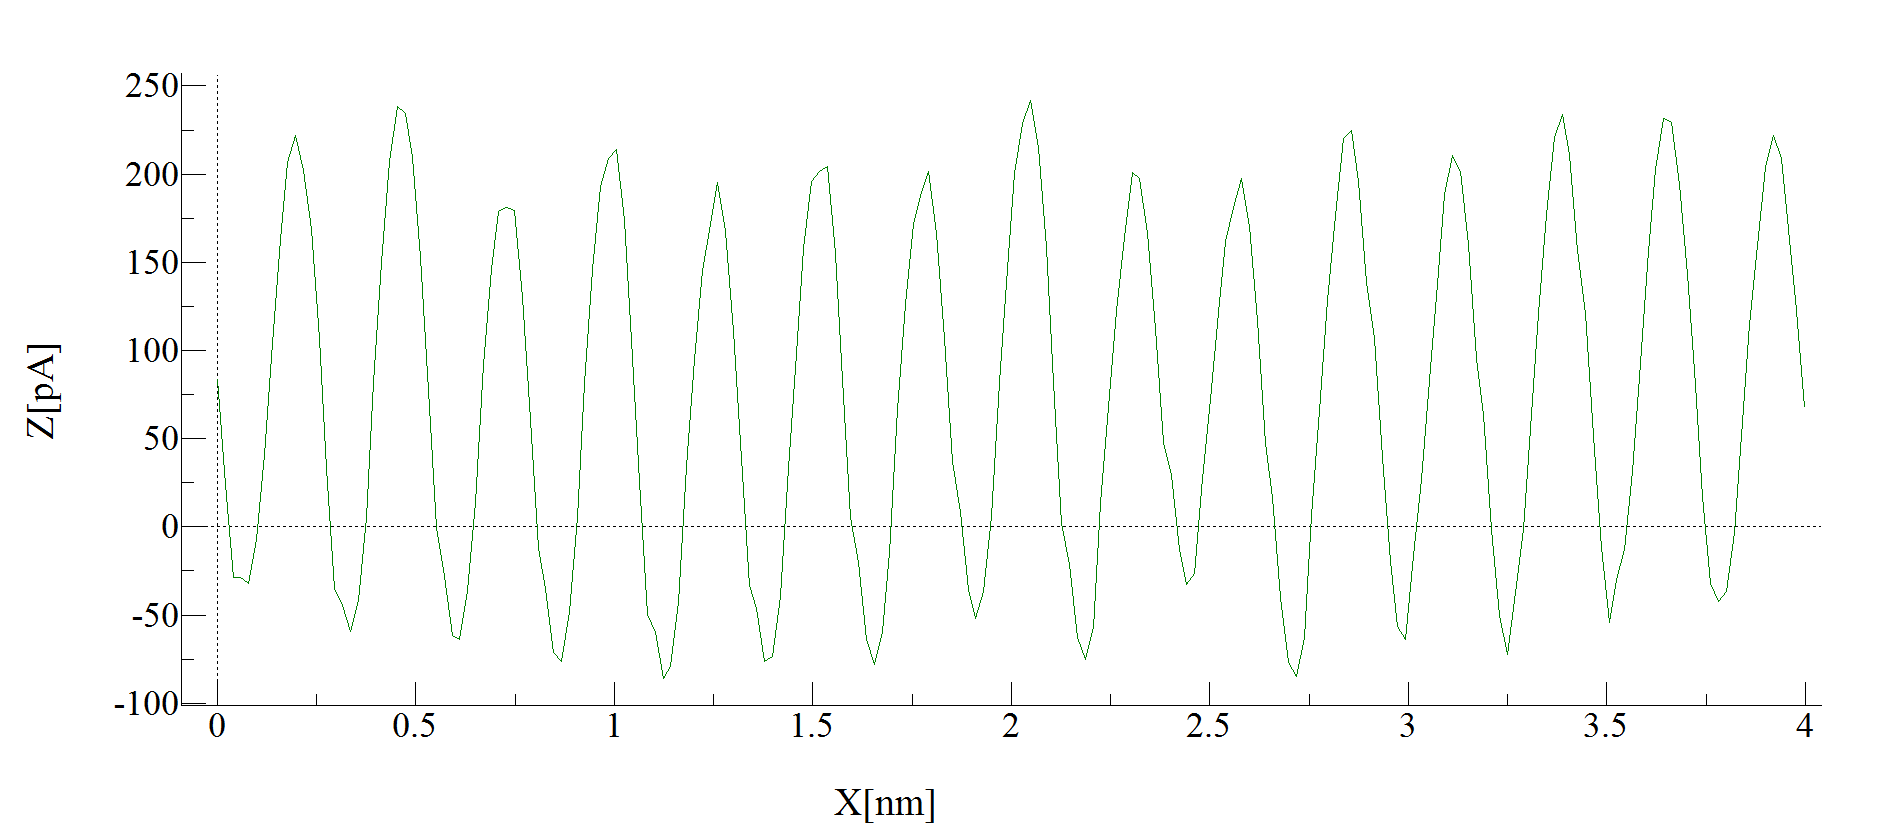
\includegraphics[scale = 0.3]{Aufnahme_Ebene_doppelte_fourier.png}
	
	\caption{Diagramm zur Messung der Abstände der atomaren Erhebungen}
	\label{Messungerh2}
\end{figure}

Zur Messung der Höhe der atomaren Erhebungen wurden die Messdaten, welche die Höhen und nicht den Tunnelstrom angeben, verwendet. Auf diesen Messdaten waren die atomaren Erhebungen selbst nach einer doppelten Fouriertransformation sehr ungenau zu erkennen, wie in Abbildung \ref{Messungerh3} zu sehen ist. Im Vergleich zu Abb. \ref{grafob2} sind die atomaren Erhebungen unschärfer und Erhebungen, die sich horizontal anordnen sind weniger abgegrenzt, als welche, die sich vertikal anordnen. Dies kommt wahrscheinlich dadurch zustande, dass der Sensor in einem Raster über die Probe fährt.

 Wir haben entlang der in Abbildung \ref{Messungerh3} zu sehenden Geraden gemessen. Das zu der Geraden gehörende Diagramm kann in Abb. \ref{Messungerh4} gesehen werden. An diesem Diagramm haben wir durch das Bilden der Differenz von Maxima und Minima die Höhen der atomaren Erhebungen gemessen. Die Werte können in Tabelle \ref{Messungerh5} gesehen werden. Nach dem Bilden eines Mittelwerts und einer Standardabweichung erhält man für den Wert der Höhe $(8,8 \pm 0,4) pm$.

Der theoretische Wert für den Abstand benachbarter Ebenen in Grafit ist $335 pm$. Dieser Wert übersteigt die von uns gemessene Höhe der atomaren Erhebungen um zwei Größenordnungen. Folglich lassen sich unsere gemessenen Höhen nicht mit diesem Wert identifizieren. Um nachzuvollziehen, wie unsere gemessenen Höhen der atomaren Erhebungen zustande kommen, müssen wir die Form der Metallspitze, die wir als Sensor benutzen, mit in Betracht ziehen. In diesem Fall betrachten wir eine einatomige Sensorspitze. Das führende Atom der Spitze hat einen gewissen Durchmesser und kann, wenn sein äußerstes Orbital ein s-Orbital ist, als eine Kugel mit gewissem Radius verstanden werden. Lässt der Tunnelstrom zwischen Sensor und Probe nach, fährt dieser näher an die Probe heran. Dies ist zum Beispiel zwischen den atomaren Erhebungen der Fall. Weil die Metallspitze jedoch einen Radius hat, wird sie, wenn sie über einer Stelle zwischen den atomaren Erhebungen ist, mit diesen beim Versuch sich der Probe anzunähern "zusammenstoßen" (Orbitale von Spitze und Probe überlappen sich). Deshalb sind die gemessenen Höhen der atomaren Erhebungen viel kleiner als der tatsächliche Ebenenabstand.

\begin{figure}[h]
	\centering
	
	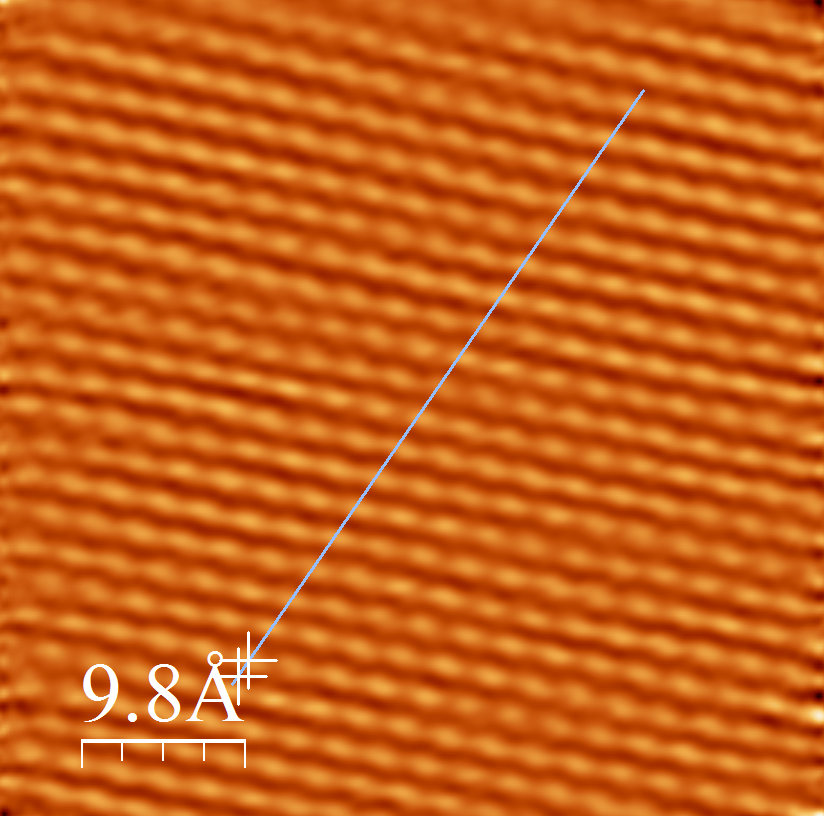
\includegraphics[scale = 0.4]{hohenmessung11.png}
	
	\caption{Messung der Höhe der atomaren Erhebungen}
	\label{Messungerh3}
\end{figure}

\begin{figure}[h]
	\centering
	
	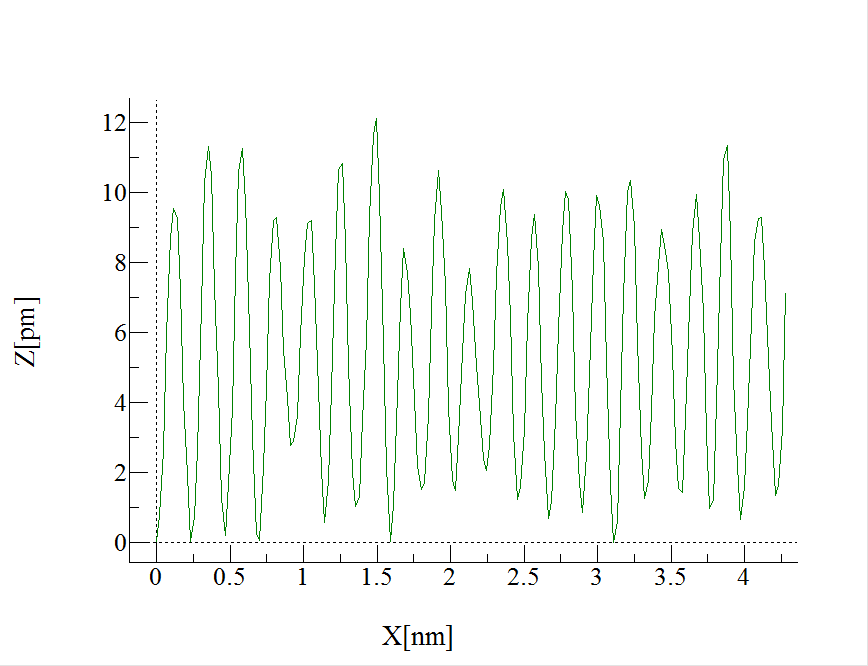
\includegraphics[scale = 0.7]{hohenmessung1_diagramm.png}
	
	\caption{Diagramm zur Messung der Höhe der atomaren Erhebungen}
	\label{Messungerh4}
\end{figure}

\begin{table}[h!]
	\centering
	\begin{tabular}{|l|l|l|l|}\hline
		Abstand & Abstand & Abstand & Höhe/pm $\pm 0,3 pm$\\
		Ausrichtung 1/nm $\pm 0,01 nm$ & Ausrichtung 2/nm $\pm 0,01 nm$ & Ausrichtung 3/nm $\pm 0,01 nm$ & \\\hline
		0,26 & 0,28 & 0,21 & 9,4 \\
		0,27 & 0,28 & 0,23 & 10,9 \\
		0,26 & 0,28 & 0,22 & 11,0\\
		0,26& 0,28 & 0,24 & 6,4 \\
		0,26 & 0,28 & 0,21 & 8,4 \\
		0,27 & 0,27 & 0,22 & 9,7 \\
		0,26 & 0,28 & 0,23 & 11,9\\
		0,27 & 0,26 & 0,20 & 6,7\\
		0,26 & 0,26 & 0,24 & 9,0\\
		0,27 & 0,27 & 0,21 & 5,7\\
		0,26 & 0,27 & 0,24 & 8,7\\
		0,28 & 0,28 & 0,21 & 8,5\\
		0,26 & 0,27 & 0,23 & 8,8\\
		0,27 &  & 0,20 & 9,6\\
		&  & 0,23 & 8,8\\
		&  & 0,24 & 7,4\\
		&  & 0,22 & 8,7\\
		&  & 0,24 & 10,2\\
		&  &  & 7,8\\
		\hline
	\end{tabular}
	\caption{Gemessene Werte für die Abstände und Höhen der atomaren Erhebungen entlang verschiedener atomarer Ausrichtungen}
	\label{Messungerh5}
\end{table}

\subsubsection{Winkel und Symmetrien} \label{winkelsec}

Anhand von Abbildung \ref{Messungerh6} haben wir die Winkel zwischen den atomaren Richtungen gemessen. Unsere gemessenen Winkel, startend von dem Winkel rechts oben und dann entgegen dem Uhrzeigersinn laufend, sind $63^\circ$, $67^\circ$, $48^\circ$, $67^\circ$, $66^\circ$ und $49^\circ$, mit jeweils einem Fehler von $1^\circ$. Wegen der hexagonalen Struktur von Grafit wäre bei einer naiven Herangehensweise zu erwarten, dass alle Winkel $60^\circ$ sind. Dies ist nicht der Fall. Es fällt auf dass die besonders kleinen Winkel($48^\circ$ und $49^\circ$) entgegengesetzt voneinander liegen. 

Die Winkel sollten nicht alle bei $60^\circ$ sein, wenn man mit dem Sensor nicht senkrecht zur Probe misst. Damit Winkel von $60^\circ$ auf $48^\circ$ heruntergehen, müsste man jedoch mit viel größeren Winkeln zum Lot auf die Probe gucken, als es bei unserem Experiment der Fall ist. Dass die Winkel von $60^\circ$ abweichen muss also eine andere Erklärung haben.

 Eine wahrscheinlichere Erklärung für die unterschiedlichen Winkel ist, dass wegen der die Probe im Raster abfahrenden Sensorspitze, das Messbild verzerrt wird. Der Sensor wird mithilfe von Piezoelementen entlang der X- und Y-Achse verschoben. Es kann sein, dass das Piezoelement, das für die Verschiebung in X- oder Y-Richtung verantwortlich ist, nicht richtig kalibriert ist. In diesem Fall fährt der Sensor nicht über die Fläche, die in den Messdaten angegeben ist. Ist zum Beispiel das Piezoelement für die y-Richtung falsch kalibriert, kann es sein, dass es eine größere Strecke abfährt, als es sollte. Weil das Programm zum Berechnen der Messbilder eine andere Strecke erwartet, wird das Messbild in y-Richtung gestaucht. Dadurch verändern sich die gemessenen Abstände und Winkel von den tatsächlichen. Durch diesen Messfehler lassen sich die bei uns von $60^\circ$ abweichenden Winkel erklären. Auch erklärt dieser Fehler, wieso die kleinsten Winkel entgegengesetzt voneinander sind.
 
 Auch der schon in Kapitel \ref{kapitolo} erklärte thermische Drift könnte eine Verzerrung der Messbilder und damit unterschiedliche Winkel zwischen den jeweiligen atomaren Ausrichtungen erklären.
 
Die von uns beobachteten atomaren Erhebungen des Grafits bilden ein hexagonales Kristallgitter. Es ist 6-zählig. Entlang einer Translation von ganzzahligen Abständen der atomaren Erhebungen der in \ref{Messungerh6} eingezeichneten Linien, gibt es außerdem eine Translationssymmetrie. Zusätzlich sieht man, dass bei einer Spiegelung entlang einer der Geraden und einer Inversion an dem Punkt, in dem sich die Geraden schneiden, das Gitter symmetrisch ist.

\begin{figure}[h]
	\centering
	
	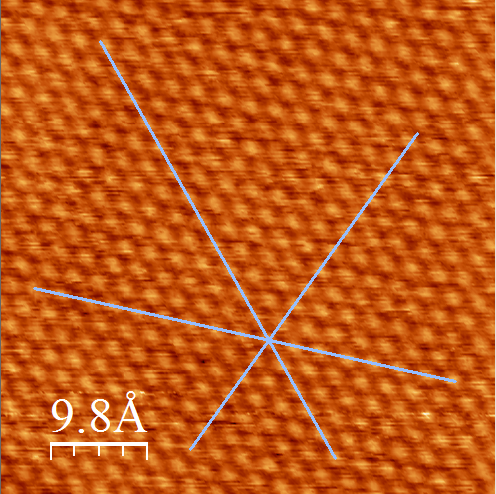
\includegraphics[scale = 0.7]{Winkelmessung_kristall.png}
	
	\caption{Messung der Winkel zwischen den atomaren Richtungen}
	\label{Messungerh6}
\end{figure}

\subsection{Fouriertransformation einer ebenen Fläche Grafits}

In Abbildung \ref{fouriertansformation_ebene} kann das Gitter aus Abbildung \ref{grafob1} nach einer Fouriertransformation betrachtet werden. Man erkennt sechs Punkte, die auf einem leicht verzerrten Hexagon um den Ursprung liegen. Um den Ursprung herum sieht man Werte in geringer Intensität. Dies sind die Störungen, die beim Aufnehmen der Messung entstanden sind. Die sechs zu erkennenden Punkte beinhalten alle Informationen über die Periodizität des gemessenen Gitters. Jedem der sechs Punkte kann ein Vektor $\vec{k}$ zugeordnet werden. Dies ist ein Wellenvektor, der eine Periodizität des Gitters angibt. Verschiebt man das Gitter also um eine Periode der Welle, die mit dem Wellenvektor $\vec{k}$ zu assoziieren ist, bleibt das Gitter unverändert. Daraus lässt sich leicht folgern, dass man aus $\vec{k}$ mit der folgenden Gleichung direkt den Abstand zweier atomarer Erhebungen berechnen kann.

\begin{equation}
	|k| = \frac{2\pi}{a}
	\label{formelk}
\end{equation}

Hier ist a der Abstand zweier atomarer Erhebungen.

Die aus Abb. \ref{fouriertansformation_ebene} mit \eqref{formelk} berechneten Werte für die Abstände der atomaren Erhebungen sind $(2,1\pm0,1)\mathring{A}$, $(2,0\pm0,1)\mathring{A}$ und $(2,5\pm0,1)\mathring{A}$. Wir haben drei Werte, weil von den sechs k-Werten jeweils zwei zu einer Periodizität gehören. Weil der Abstand der atomaren Erhebungen entlang aller atomaren Ausrichtungen gleich groß sein sollte, wäre auch zu erwarten, dass in der Fourierdarstellung alle gemessenen k-Werte gleich groß sind. Wegen der Verzerrung der Messbilder, sind die k-Werte jedoch unterschiedlich. Der dadurch entstehende Fehler für die Berechnung der atomaren Abstände in größer, als der direkte Messfehler aus dem Messbild. 
Nur einer der drei Messwerte stimmt mit kleiner gleich drei Fehlerintervallen mit dem theoretischen Wert von $2,46\mathring{A}$ überein.
Um gute Messwerte für die atomaren Abstände zu erhalten, müsste man die Verzerrung der Messbilder entfernen.

%Deshalb geben wir den mithilfe der k-Vektoren berechneten Wert der Abstände der atomaren Erhebungen als Durchschnittswert mit der Standardabweichung als Fehler an. Der berechnete Wert ist $(2,2 \pm 0,3)\mathring{A}$. Er stimmt mit den in \eqref{eq:aabstand} theoretisch berechneten Wert von $2,46\mathring{A}$ überein. Es scheint, dass sich wegen der Verzerrung der Messbilder, die Fourierdarstellung des Gitters weitaus besser zum Bestimmen das Abstands der atomaren Abstände eignet, als das direkte Ausmessen in den Messbildern.

\begin{figure}[h]
	\centering
	
	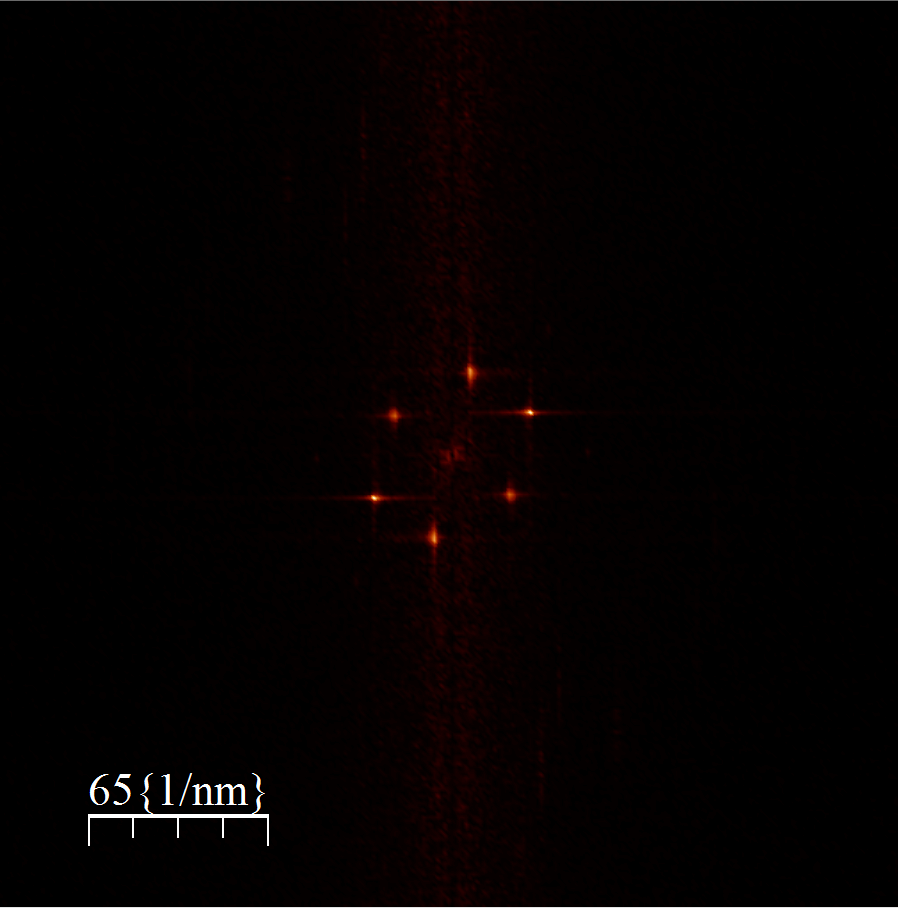
\includegraphics[scale = 0.5]{Fouriertrasformation_kristall.png}
	
	\caption{Fouriertransformation von Abbildung \ref{grafob1}}
	\label{fouriertansformation_ebene}
\end{figure}

\section{Diskussion}

Wir haben mit dem Rastertunnelmikroskop die Struktur von Grafit betrachtet. Da unsere Sensorspitze nicht fein genug war, konnten wir zwar Kanten an der Oberfläche, die atomare Struktur des Grafits jedoch nicht erkennen, beziehungsweise nur eingeschränkt über eine kleine Fläche. Deshalb mussten wir zur Betrachtung der Struktur von Grafit Referenzmessungen benutzen.

Anhand der Referenzdaten untersuchten wir die hexagonale Struktur des Grafits. Es konnten Translations-, Inversions-, Spiegelungs- und Rotationssymmetrien erkannt werden. Die leicht unterschiedlichen Größen der Winkel zwischen den atomaren Richtungen konnten wir damit erklären, dass das X- oder Y-Piezoelement zum Bewegen des Sensors nicht richtig kalibriert war.

Unsere aus den Messbildern abgelesenen Werte für die Abstände der atomaren Erhebungen waren entlang der verschiedenen atomaren Ausrichtungen $(2,7 \pm 0,1) \mathring{A}$, $(2,7 \pm 0,1) \mathring{A}$ und $(2,2 \pm 0,1) \mathring{A}$. Sie wichen mit 3 Fehlerintervallen von dem theoretischen Wert von $2,46 \mathring{A}$ ab. Es erwies sich, dass sich die Abstände mithilfe einer Fouriertransformation besser bestimmen ließen. Die aus der Fouriertransformation bestimmten Werte waren $(2,1\pm0,1)\mathring{A}$, $(2,0\pm0,1)\mathring{A}$ und $(2,5\pm0,1)\mathring{A}$. Einer der Werte stimmt mit dem theoretischen überein, während die anderen Werte über 3 Fehlerintervalle von ihm abweichen.
 Auch wenn die Werte aus der Fouriertransformation nur zum Teil bessere Ergebnisse, als die aus den Messbildern liefern, ist ihr Fehler besser einzuschätzen. Die Verzerrung der Messbilder kann sofort bei Betrachtung der Fourierdarstellung erkannt werden. Bei einer direkten Betrachtung der Messbilder war die Verzerrung erst nach dem Ausmessen der Winkel zwischen den atomaren Ausrichtungen oder dem Berechnen der Abstände der atomaren Erhebungen zu erkennen.

Bei einer richtigen Kalibrierung des X- und Y-Piezoelements könnte man eine Verzerrung der periodischen Strukturen des Gitters verhindern. Dadurch könnte man die Messung der atomaren Abstände anhand der Fourierdarstellung präziser und mit kleinerem Messfehler durchführen. Eine numerische Lösung der Verzerrung wäre möglich, jedoch mit hohem Aufwand verbunden.
Es ist nicht auszuschließen, dass die Verzerrung der Messbilder möglicherweise nicht durch falsch kalibrierte Piezoelemente, sondern durch den thermischen Drift zustande kommt.

Um bessere Versuchsergebnisse zu erzielen, könnte man die Sensorspitze des Rastertunnelmikroskops mit einer anderen Methode herstellen. Die Feinheit der Sensorspitze ist für den Erfolg des Versuchs ausschlaggebend und bestimmt, ob es möglich sein wird, die atomare Struktur des Grafits zu messen.

\end{document}